\documentclass[12pt]{article}
\usepackage{amsmath}%
\usepackage{amssymb}%
\usepackage{multicol}
\usepackage{graphicx,epsfig}%
\usepackage[margin=1in]{geometry}
\usepackage{rotating}%
\usepackage{url}
\usepackage[backend=bibtex, citestyle=ieee]{biblatex}
\bibliography{paper}
\usepackage{epsfig}%
\usepackage{epstopdf}%
\usepackage{varwidth}
\usepackage{lscape}%
\usepackage{color}
\usepackage[hang,flushmargin]{footmisc} 
\pdfminorversion 3
\usepackage{pbox}

\usepackage{subfig}

\newcommand{\hilt}[1]{\colorbox{green}{#1}}
\usepackage{setspace}
\usepackage{adjustbox}
\def\x{\mathbf{x}}

\newcommand\blfootnote[1]{%
  \begingroup
  \renewcommand\thefootnote{}\footnote{#1}%
  \addtocounter{footnote}{-1}%
  \endgroup
}

\newcommand{\tcr}{\textcolor{red}}
\newcommand{\tcb}{\textcolor{blue}}
\newcommand\tab[1][1cm]{\hspace*{#1}}

\DeclareMathOperator*{\argmin}{argmin} 
\renewcommand{\baselinestretch}{1.5}
\usepackage{tabularx}

\setcounter{tocdepth}{4}
\setcounter{secnumdepth}{4}

\usepackage{bibentry}

\usepackage{listings}

\definecolor{lightgray}{gray}{0.9}

\lstset{
    showstringspaces=false,
    basicstyle=\ttfamily,
    keywordstyle=\color{blue},
    commentstyle=\color[grey]{0.6},
    stringstyle=\color[RGB]{255,150,75}
}

\newcommand{\inlinecode}[2]{\colorbox{lightgray}{\lstinline[language=#1]$#2$}}

\title{S19: REU Research Document}
\author{Emily Slaughter, Gennie Mansi }

\begin{document}

\maketitle

\clearpage

\tableofcontents

\clearpage

%%%%%%%%%%%%%%%%%%%
\section{Abstract} \label{abstract}

The term design rules refers to the choices about the design of a project and how those choices are implemented. Design rules are integral in maintaining project coherency and forwards and backwards compatibility. Documentation is critical to preserving information about design rules. However, most documentation is not updated frequently, and only individual developers know critical pieces of information. We developed an algorithm that can represent the information contained in a code base and automatically suggest likely design rules. Our results demonstrate that our algorithm can successfully represent and identify significant design rules, and has the potential to be used to automatically generate documentation for a project.



\clearpage
%%%%%%%%%%%%%%%%%%%
\section{Introduction} \label{intro}

Proper documentation forms an integral part of developing and maintaining software, especially given the increasing size of code bases and the prevalence of temporally and spatially dispersed developers. As code is written and a project develops, various design decisions are made, which impact both existing and future code. Documentation of design decisions and the rationale behind those decisions is dependent on the developer and is often recorded or dispersed between several disparate locations, including a formal document, comments in the code, and the developers themselves. However, documentation is often not written, read, or updated, causing developers to depend largely on the code and other sources of information rather than explicit, written documentation. 

Ideally, as code is authored or modified, it should follow design rules that were previously used to author code. The \textit{design rules} for a project are the set of choices about the code's design and how those choices are implemented. Several sources of information, including search history, cursor location, event logs, debugger information, and the code itself can indicate what elements in the code base are most pertinent to the user and are most likely to contain design rules of interest. Some information about design rules may only be recorded in the memories of co-workers, and thus access to this kind of information is also critical for developers trying to understand and use existing code. 

Mixed human-AI authoring of code patterns can greatly assist developers to efficiently and accurately develop and maintain a unified set of rules. There are an infinite number of patterns that could be found in a given code base, and an even larger diversity of representations for those patterns; therefore, the crux of the problem lies in determining how to represent the information contained in the code base and in identifying the patterns using the chosen representation. Hence our focus is on mining design rules from a given code base in any language in order to facilitate active documentation and maintenance of code.

We explore how information from outside of the code base could be used to inform what patterns are identified. We seek to develop a tool that combines both automatic and manual rule-authoring capabilities. It should also automatically provide live updates with examples and violations of authored design rules. Ultimately, such a tool will greatly increase the amount of up-to-date documentation available to developers.

The rest of the paper is organized as follows. Section~\ref{methods} contains assumptions that are made about developers, a discussion of the different sources of information about design rules that are available, and a description of our algorithm. We discuss our three different approaches to representing the components of design rules in Section~\ref{algm_attrApproaches}. Section~\ref{results} contains a description of the results for our algorithm, followed by a description of the tool interface in Section~\ref{toolInterface}. Finally, we discuss the short comings of our algorithm and related in works in Sections~\ref{relatedWorks} and Sections~\ref{disc}, respectively.
 
 
 \clearpage


%%%%%%%%%%%%%%%%%%%
\section{Methods}\label{methods}

\subsection{Problem Description} \label{probDesc}

Given the code for a project and some external information such as cursor information, we wish to derive a set of most likely and relevant design rules. We will then integrate our algorithm for mining these design rules into an interface that allows developers to seamlessly mine and write design rules and to see violations and correct examples of these rules. 

When considering our task, there exist two significant considerations: (a) what kinds of data are available and helpful for suggesting rules, and (b) what kind of algorithm can be utilized with these sources of data in order to make relevant design rule suggestions. We will begin by first addressing different sources of information that are available and most useful for our purpose. Then, we will proceed to discuss our algorithm for design rule mining.


\subsection{Assumptions about the user} \label{assumptions}

Developers can be divided into three categories with respect to their familiarity with a project or code base. First, a developer may be experienced with a given code base. She would have a thorough understanding of the project, its objectives, and its implementation. She is in a position that allows her to author design rules and verify that certain rules have been followed throughout the project. Second, a developer may be partially knowledgable about a project and its implementation. Such a developer may have a general familiarity with the code and its implementations, but is not able to easily or confidently author design rules or may simply wish to explore possible existing design rules. On her own she is not be able to produce an accurate rule, but she might be able to see a rule and provide useful feedback on its correctness or relevancy. Finally, a developer may be completely unfamiliar with a code base. Existing design rules and documents would be extremely helpful in helping her understand the structure of the code. She may also need to frequently consult co-workers about code standards and patterns if there is a significant lack of written documentation. In such a situation, the developer may even be interested in looking for examples on what kind of existing design rules to which she should adhere.

 Work has already been completed with regards to the first category, and while much research has been done in code suggestion, completely automated design rule generation seems largely unexplored (see Section~\ref{relatedWorks}). Therefore, an algorithm developed with the second category of developers in mind forms a natural bridge between human authored design rules and completely automated rule authoring. Consequently, we assume the developers for which we are designing our algorithm have some general familiarity with the code and can identify proper design rules if supplied with a set of rules to consider. Thus, feedback form the developer about hypothesized rules is dependable, enabling mixed human-AI rule authoring.


\subsection{Sources of Information} \label{infoSrcs}

	Part of knowing which sources are most useful for deriving information about design rules is understanding where developers themselves look for information about a project and what kinds of information are useful to programmers.  

Several studies have demonstrated that as developers work and explore a project, they try to answer high-level questions about what, why, and how code causes different program states as they try to complete a task \cite{SadowskiEtAl2015, LaTozaMyers2010, LaTozaEtAl2007}. Researchers who investigated how programmers read and explore code have found that programmers' activities include checking implementation details, checking common style, and browsing. Programmers also performed code search to understand various dependencies within and between projects, why something is failing, and the side effects of a proposed changed \cite{SadowskiEtAl2015}. 

Ko et al investigate what sources of information developers use to accomplish a task and how that information affects developers' workflow throughout the day. They report that developers look at a variety of sources to accomplish a task, including check-in logs, bug reports, content management systems, version control systems, and other coworkers. Additionally, they identify knowledge about design and program behavior as the type of information that is most often deferred since unavailable coworkers are often the only source of knowledge. Developers sought out coworkers most often when there were information needs with regards to code design. Other questions to coworkers centered around following the team's conventions. Developers asked specific questions regarding what code caused different program states and behaviors and what statically related to the code of interest, but pursued the answers to these questions by starting with a hypothesis that they largely developed by using their intuition, asking coworkers, looking for execution logs, scouring bug reports, and using the debugger. They then often refined their hypothesis by using the search tool to answer questions about which sections of code performed similar operations \cite{KoEtAl2007}. 

Furthermore, Fritz et al conducted a survey of nineteen professional Java programmers in order to generate a degree of interest model to reflect developers' knowledge of code \cite{FritzEtAl2007}. The researchers' model was based on the total number of interactions the programmer has with an element and the recency of that interaction. Other factors they identified that could be used to improve their model included authorship of program elements, the role of elements, and the task being performed \cite{FritzEtAl2007}.

Based off of  these findings, we can conclude that there are a variety of pertinent and accessible sources of information for our algorithm, including the debugger, code base, cursor location and search histories, and the developer herself. However, we focus on trying to find rules using only the code base and direct feedback from the developer. The reason for this decision is that the code base and direct feedback are the only two sources of information that we are guaranteed. Future iterations of this algorithm may also use these other sources of information to generate design rules.

\subsection{Representing the code base and design rules}
Our representation of the features in the code base ultimately impacts the way that we identify design rules. Ideally, we would output information only about the most critical features of the code base that can lead us to the most likely design rules. However, the code base contains a lot of information and there are many ways of representing that information. Additionally, there are scalability concerns since code bases can easily have over a quarter million lines of code. Ultimately, our representation of the features of the code base is linked to the way that design rules can be represented.

Design rules can be represented as ``IF/THEN" statements where \textit{IF} some quality is true about a section of code \textit{THEN} some condition is applied. We represent different features of the code using \textit{attributes}. An attribute is a way of representing some feature(s) of the code. Thus, we can decompose design rules into a set of attributes. The ability to group attributes into ``IF" attributes and ``THEN" attributes would enable us to generate design rules. Our goal then is to associate different attributes about the code base, so we can synthesize them to create design rules. 

The challenge then is what kinds of attributes to generate (that is, what kinds of representations for the code to use), since there are many different ways to represent the features of a code base (see Figure~\ref{fig:attrEx}). Consequently, there are many ways to represent a design rule (Figure~\ref{fig:drEx}). 

\begin{figure}[h!]
  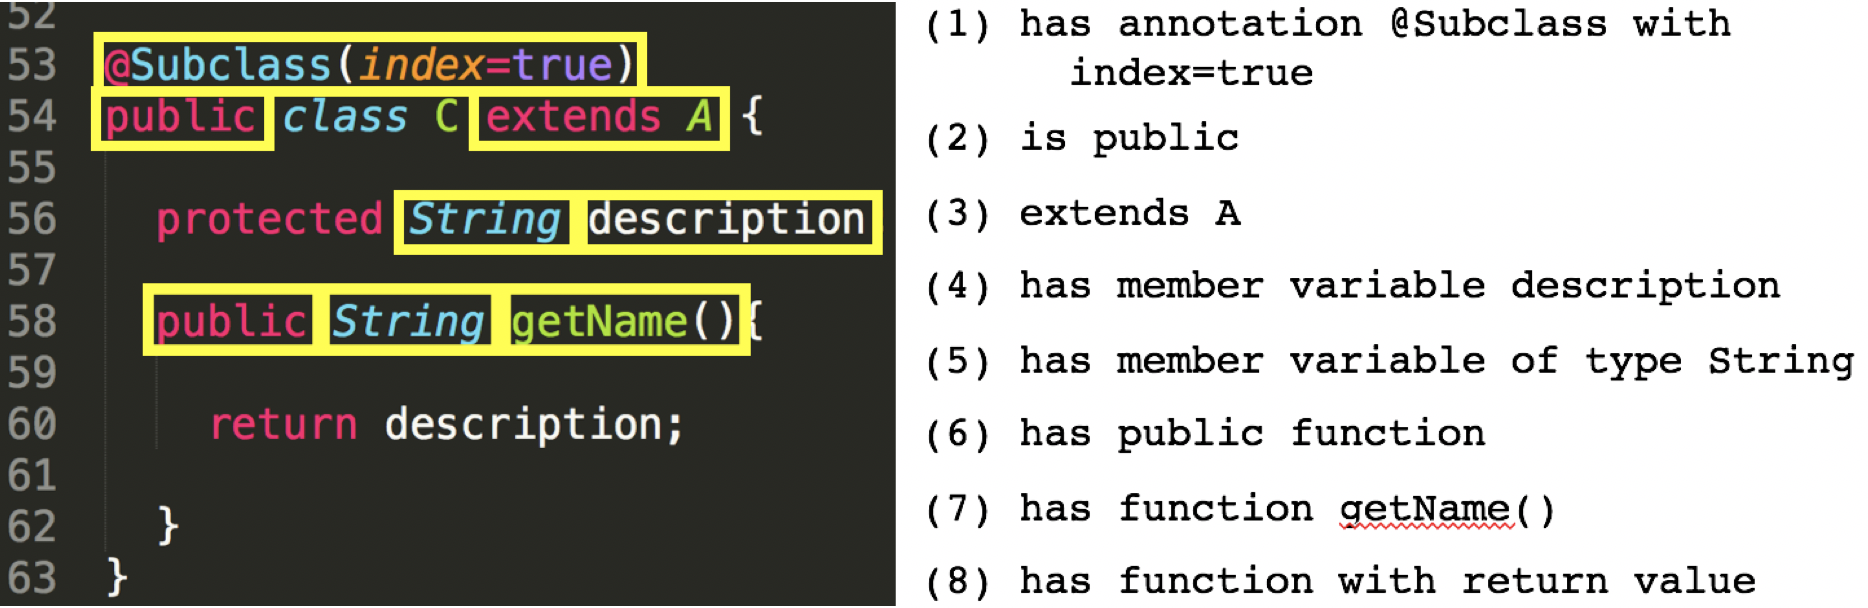
\includegraphics[width=\linewidth]{attributeEx.png}
  \caption{There are many different attributes that can be created that represent different features of the code in different ways.}
  \label{fig:attrEx}
\end{figure}



\begin{figure}
  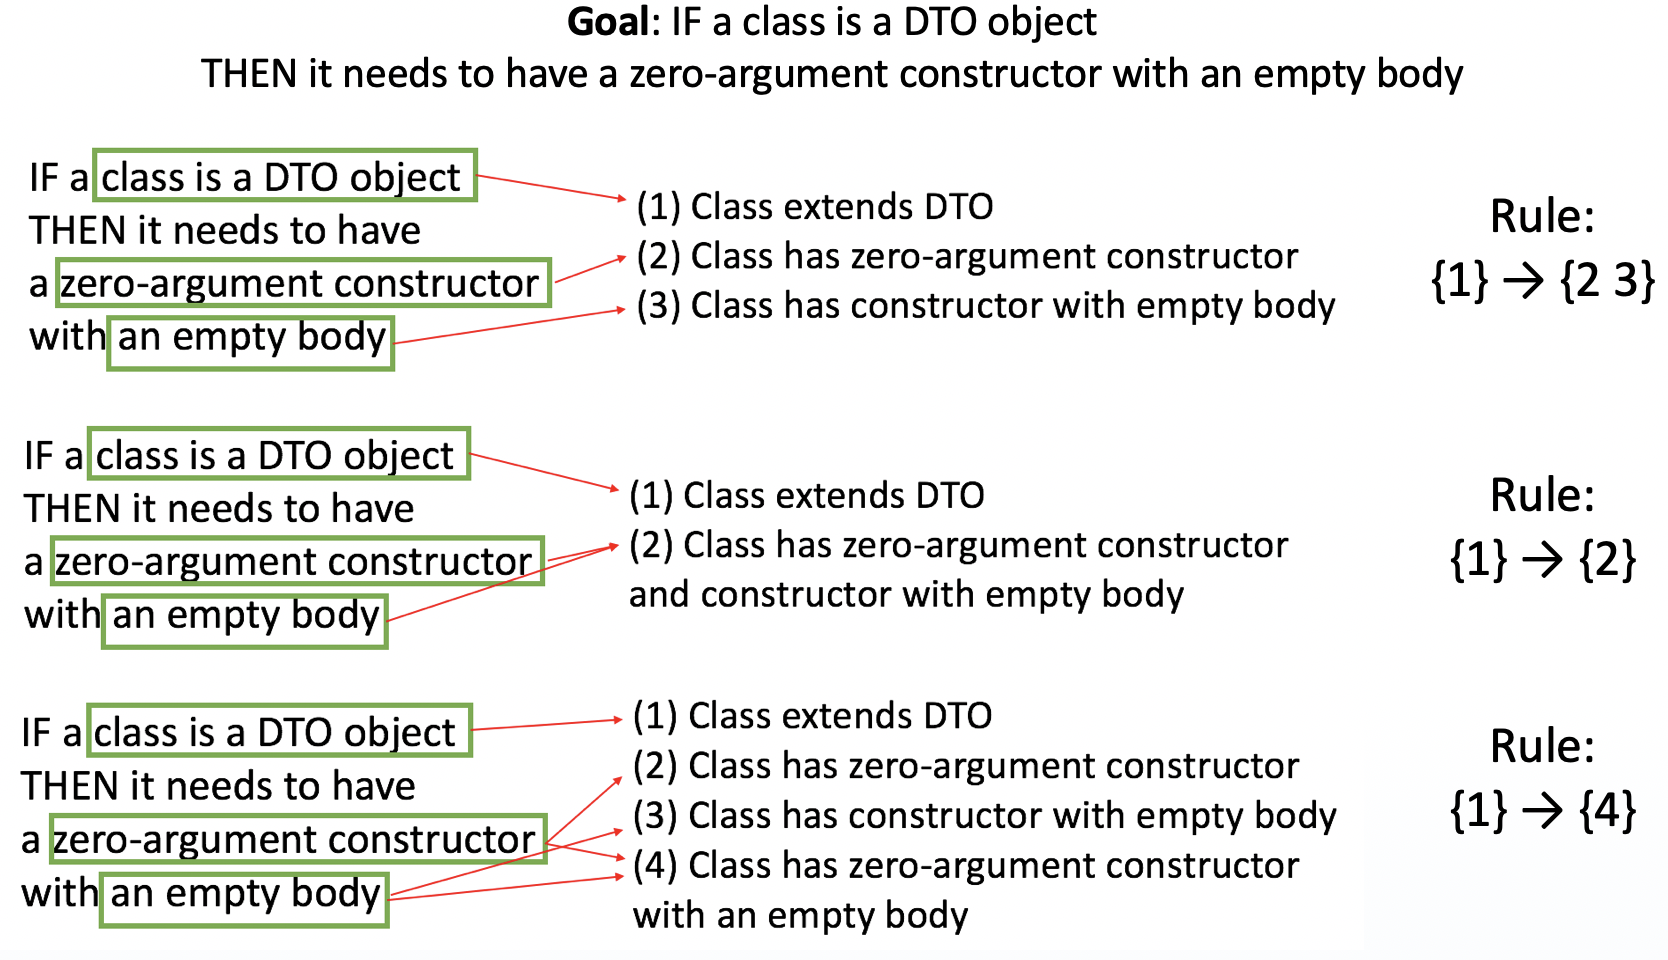
\includegraphics[width=\linewidth]{designRuleEx.png}
  \caption{Notice that from the same segment of code, we have many different ways of representing the corresponding design rule.}
  \label{fig:drEx}
\end{figure}





\subsection{Algorithm} \label{algm}

\subsubsection{Outputting the attributes}\label{algm_attrApproaches}

We approached outputting attributes in three different ways, all of which we present in Section~\ref{algm} and analyze in Section~\ref{results}. Figure~\ref{fig:attrFunction}, ~\ref{fig:attrConstructor}, ~\ref{fig:attrField}, and ~\ref{fig:attrClass} contain a summary of the different kinds of attributes output by each of these algorithms. For all four of these figures, yellow dots represent Approach 1, green dots represent Approach 2, and orange dots represent Approach 3.

	\paragraph{Approach 1}
	
	The basic idea in this approach is that we would have a set of reserved item IDs corresponding to “default” attributes that we know we always have a chance of finding. For example, there is always the chance that there is a public class; thus, there is a reserved item ID corresponding to an attribute titled “is a public class”. We also output attributes that are specialized to the code base from which they are derived, such as annotations that are on classes and what classes are involved in an inheritance structure. Each line output to the database represented the set of attributes belonging to a different class in the code base.

	\paragraph{Approach 2}
	
	The second approach entailed generating several databases that could be further mined for more detailed information. The logic behind this approach is that it might be easier to output more specific attributes for different subsets of the data that are related, and thus find more specific and interesting rules. Each starting database would have rows composed of different subsets of the data that are related. For example, one database might contain more specific attributes related to subclasses, with each row in the database representing a different subclass. Other output databases may have rows composed of the different functions in a class, and another would have rows representing different subclasses. Once these databases are generated, association rules would be derived from them. Based off the association rules that are created, a second more detailed database might be created in order to mine more specific information about the rule. For example, the database with rows made from distinct functions might generate a rule that says “IF there is a function that returns the call from a constructor 
THEN it needs to return a specific type $<$type name$>$.” The second database created would be composed of rows all of which are functions that return the call from a constructor and return the specific type. Attributes for the derived database could include more specific characteristics about the constructor, such as the parameters required by the constructor and the type of object created by the constructor. Then, if needed, a tertiary, more specific database could be output with even more specific attributes.

	\paragraph{Approach 3}
	
	Our third approach entails outputting more detailed attributes about subsets of the code base and analyzing the attributes found in the subsets for design rules. For each subset of the code base, we have a \textit{focus} class from which a set of global attributes is created; any class in the subset that is not the focus class is a \textit{peripheral} class. Only the attributes found in both the focus class and peripheral classes are output. The main advantage to outputting the attributes in classes this way is that it is more scalable. Since the set of global attributes is compiled only of the attributes of a single class, a greater number of attributes can be output without significantly decreasing efficiency or scalability.
	
	The attributes that are output are a mix of more and less detailed attributes about subsets of the different classes in the code base. Many of the same attributes are output by both this approach and Approach 1. However, in this approach we also output more specific attributes that contain information about multiple features. Attributes specifically include annotations on classes, functions, and fields complete with the annotation name and arguments, constructors storing all of the values passed as arguments in member variables, constructors having empty bodies or non-empty bodies, the return types of functions. 
	


\begin{figure}
\centering
\parbox{8 cm}{
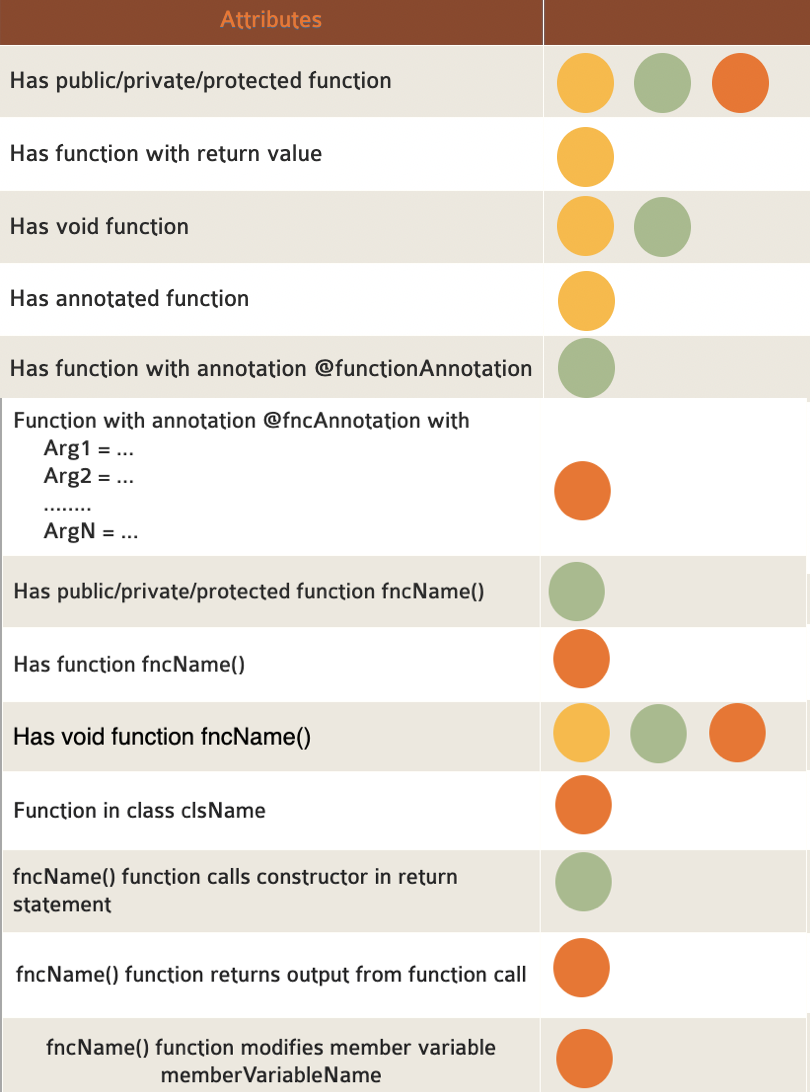
\includegraphics[width=\linewidth]{attributeFunctions.png}
\caption{A comparison of the attributes regarding functions produced by Approach 1, 2, and 3.}
\label{fig:attrFunction}}
\qquad
\begin{minipage}{7.5 cm}
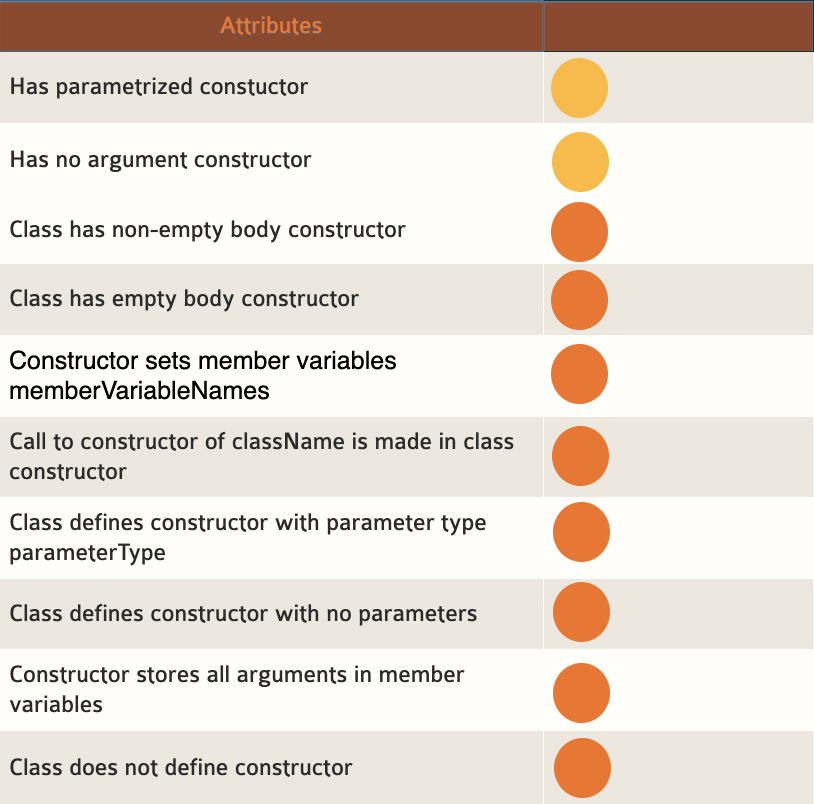
\includegraphics[width=\linewidth]{attributeConstructors.png}
\caption{A comparison of the attributes regarding constructors produced by Approach 1, 2, and 3.}
\label{fig:attrConstructor}
\end{minipage}
\end{figure}

\makebox[\textwidth]{attributeFunctions.png}



\begin{figure}
\centering
\parbox{7.5 cm}{
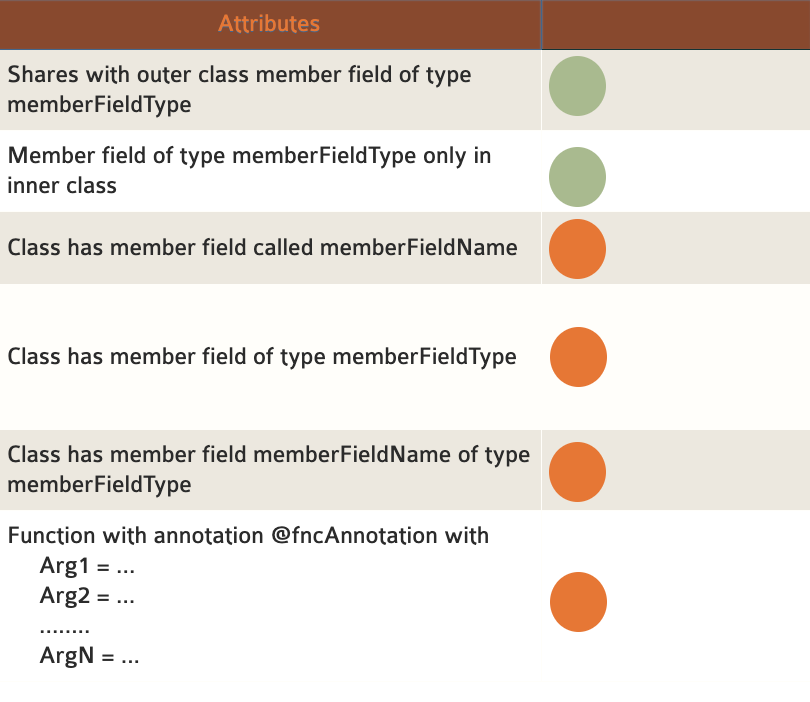
\includegraphics[width=\linewidth]{attributeFields.png}
\caption{A comparison of the attributes regarding functions produced by Approach 1, 2, and 3.}
\label{fig:attrField}}
\qquad
\begin{minipage}{8 cm}
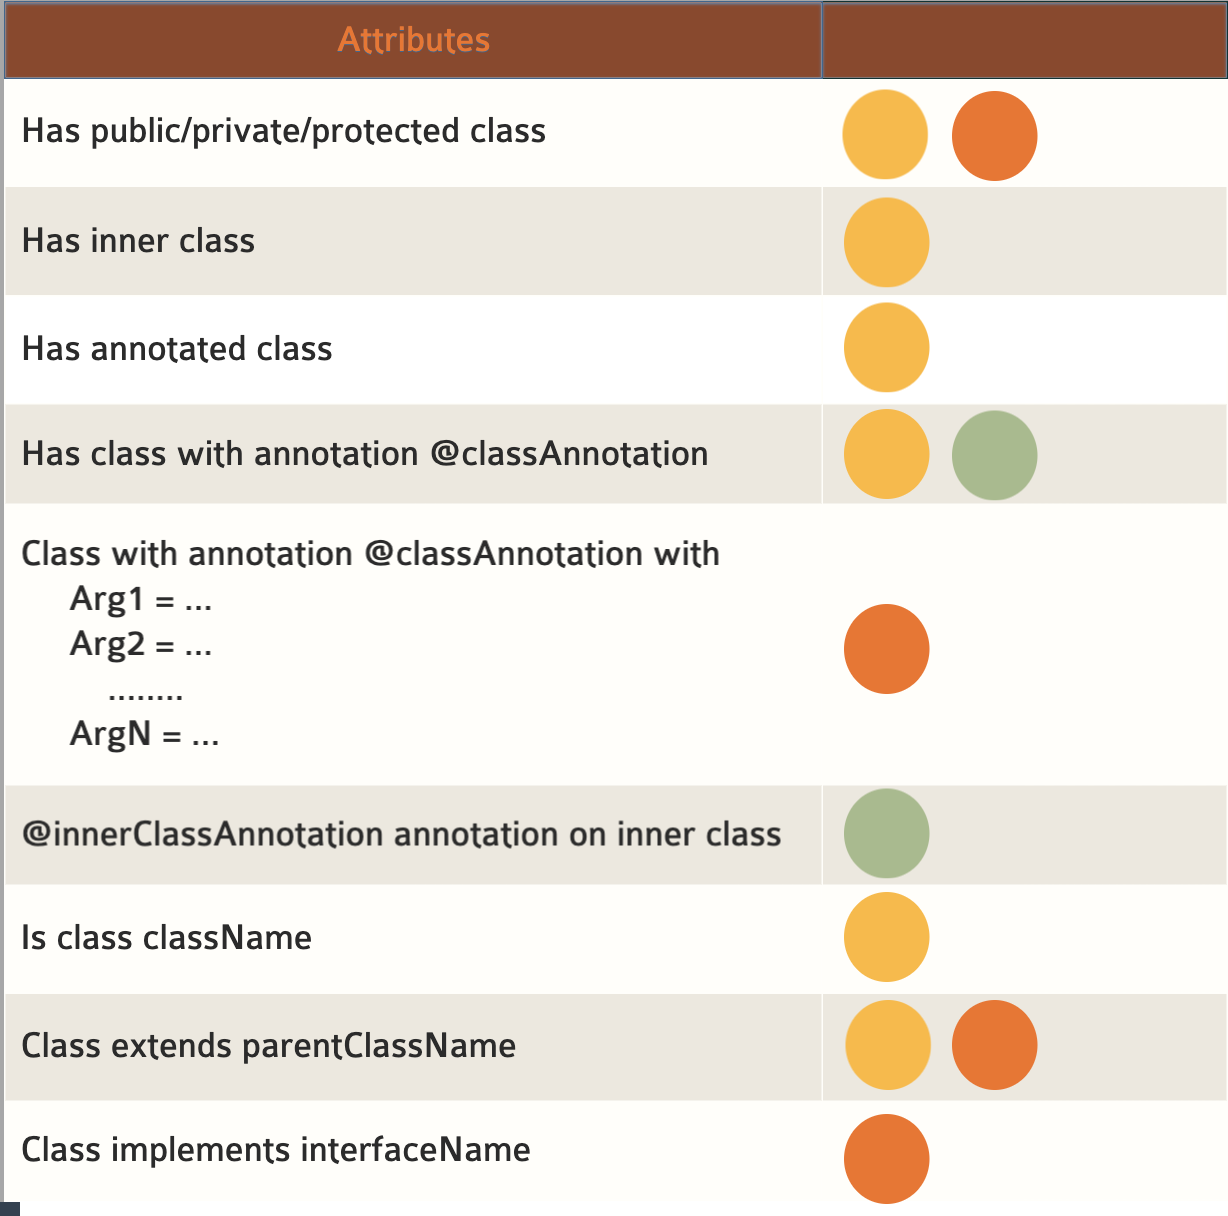
\includegraphics[width=\linewidth]{attributeClass.png}
\caption{A comparison of the attributes regarding constructors produced by Approach 1, 2, and 3.}
\label{fig:attrClass}
\end{minipage}
\end{figure}


	
	
\subsubsection{Associating attributes}
	We chose the Frequent-Pattern (FP) Growth Algorithm, which is an algorithm frequently used in association rule mining (ARM). ARM seeks to mine databases for patterns of items that frequently occur together. It is often used in market basket analysis to see what products are often purchased simultaneously. FP Growth is a type of association rule mining algorithm that efficiently finds frequent itemsets (FIs) by storing their patterns in a tree data structure. Advantages of the FP Growth algorithm include:
	\begin{itemize}
		\item It’s designed to find hidden patterns among items.
		\item Its scalability and relative efficiency.
		\item Various implementations that deal with sparse data already exist.
	\end{itemize}
In our case, the items in the FIs output by the algorithm are groups of attributes that frequently appear together in the code base.

There are two notions of frequency that are used in FP-Growth and other ARM techniques:
	\begin{enumerate}
		\item Support - the joint probability of two or more items.
		\item Confidence - the conditional probability of two or more items.
	\end{enumerate} 
Both are typically expressed as percentages ranging from 0-100\%, and are used to produce FIs that occur with a particular frequency. The support and frequency are used to fine tune the algorithm and varying them can result in finding different FIs.

\subsubsection{Generating candidate design rules}

Once the FIs have been produced an extension of the algorithm produces association rules. Items in an association rule are either in the antecedent (``IF") portion of the rule or the consequent (``THEN") portion of the rule. Rules are interpreted, ``IF (\textit{insert antecedent}) THEN also (\textit{antecedents}) tend to be present". We use the association rules produced from the algorithm as our candidate design rules to present to the developer.


\subsubsection{Selecting queries to present to user}

\tcr{[Work in progress]}

\clearpage

%%%%%%%%%%%%%%%%%%%
\section{Results} \label{results}
In order to assess our success in identifying “interesting” rules, we used a set of sample design rules written for a java-based project called CrowdCode. CrowdCode is a program designed to help groups of developers delegate and keep track of tasks for large coding projects and software. For each approach discussed in Section~\ref{algm}, we analyze how well we could reproduce the sample design rules for CrowdCode as well as scalability concerns.

	\subsection{Approach 1}
	This approach was not successful even when used with lower support (20-40\%). The general problem was that associations produced from this database were uninteresting and obvious. For example, many of the rules produced were rules such as, “IF it is a public class THEN it has a public function” or “IF it is a class with annotation @$<$class name$>$ THEN it is a class that has an annotation”. 

The reason such association rules were output is due to the fact that all the attributes were fairly general, and many default attributes overlapped with more specific attributes, such as the above example with annotations. These overlapping attributes always occurred together, and thus most of the rules FP-Growth produced were made of overlapping attributes. Hence, more interesting rules could not be discovered.

	\subsection{Approach 2}
	The main prohibiting factor in this approach, is the total number of tables created and the total number of times the code would need to be traversed to create all of the tables. Consequently, we found this approach to be impractical, and did not seek to pursue this approach further.

	\subsection{Approach 3}
	
	We explored 6 different groups of files to test if we could find the attributes of interest. The focus class was chosen as the class with the largest file size that was not the parent class if there was an inheritance structure. We present the groups of classes that were successfully used to identify one of our target design rules. Under each group of classes, we list the rules that we found along with an explanation. A discussion of what rules could not be discovered and why follows this portion. Supplementary material contains the output for all six groupings. 
	
	\subsubsection{Command classes}
		This group included classes that extended the Command class and the Command class itself. The focus class for this group was \inlinecode{Java}{QuestioningCommand.java}.
		
		\paragraph {Rules found}
			
			\subparagraph{Commands must implement execute} IF a class is a subclass of Command THEN it must implement execute.
			
			The attributes of interest that are generated here are (1) class extends Command, (2) has public function execute(), (3) has void function execute(). We output both these attributes, so we should be able to find them together in frequent itemsets. We used support 60\% and confidence 80\% for all our tests. 
		\begin{itemize}
			\item (1) and (2) were found together in approximately 22\% of all FIs.
			\item (1) and (3) were found together in approximately 12\% of all FIs.
			\item (1), (2), and (3) were found together in approximately 6\% of all FIs.				\item (2) and (3) were found together in approximately 12.5\% of all FIs. 
		\end{itemize}
		
			\subparagraph{Commands should persist all data they are given.} IF a constructor is for a subclass of Command THEN it should store each parameter given. 
			
			The attributes of interest that we represent are (1) class extends command and (2) constructor stores each parameter given. We used support 60\% and confidence 80\% for all our tests. Both attributes were found in about 24\% of all FIs.
			
				
	\subsubsection{Classes and subclasses that extend DTO }
		This group included classes that extended the DTO class and the subclasses of the classes that extended the DTO class. The focus class for this group was \inlinecode{Java}{FunctionInFirebase.java}.
		
		\paragraph {Rules found}
		
		\subparagraph{DTOs must have a zero-argument constructor.} IF a class is a DTO object THEN it needs to have a zero-argument constructor with an empty body.
		
		The attributes of interest are (1) class extends DTO, (2) class has zero-args constructor, and (3) class has empty body. With 60\% support and 80\% confidence, these three attributes were found in 6.5\% of the FIs.

	
	\subsubsection{Classes, subclasses, and sub-subclasses that extend DTO}
		This group included classes that extended the DTO class and the subclasses and sub-subclasses of the classes that extended the DTO class. The focus class for this group was  \inlinecode{Java}{FunctionInFirebase.java}.
		

		\paragraph {Rules found}
		
		\subparagraph{DTOs must have a zero-argument constructor.} IF a class is a DTO object THEN it needs to have a zero-argument constructor with an empty body.
		
		The attributes of interest are (1) class extends DTO, (2) class has zero-args constructor, and (3) class has empty body. With 60\% support and 80\% confidence, these three attributes were found in 5.1\% of the FIs.
		
		
	\subsubsection{@Entity classes}
		This group included all the classes that had the @Enitty notation placed directly above them. The focus class for this group was \inlinecode{Java}{Project.java}.
		\paragraph {Rules found}
		
		\subparagraph{@Entity classes must have an @id field.} IF a class has an @Entity annotation THEN it must have a field annotated with @Id. 
		
		The attributes of interest are (1) class has @Entity notation and (2) member field has annotation @id. With 50\% support and 80\% confidence, approximately 22\% of all FIs generated by the FP growth algorithm contained these two attributes.
		
		\subparagraph{Subclasses of @Entity classes must be indexed.} IF a class is a subclass of an @Entity class THEN it needs to be indexed ('index=true'). \tcr{[I couldn't find exact numbers on what percentages were output for these groupings.]}
		
		\subparagraph{@Entity classes must have a zero-argument constructor.} IF a class is an entity THEN it needs to have a zero-argument constructor.
		
		The attributes of interest are (1) has @Entity annotation and (2) class has zero-args constructor. With 60\% support and 80\% confidence, approximately 20\% of the FIs generated by the FP growth algorithm contained these two attributes; as a side note, if support was lowered to 50\%, then approximately 23\% of the FIs generated contained both attributes.



	\subsubsection{Artifact classes }
		This group included all the classes that extended the Artifact class. The focus class for this group was \inlinecode{Java}{Function.java}.  

		\paragraph {Rules found}
		
		\subparagraph{Artifacts should be marked as a data region with an @Entity annotation}.  IF an object is an artifact subclass THEN it needs to be an entity.

		In this case, the attributes of interest are ``extends Artifact” and ``class has @Entity annotation”. With 60\% support and 80\% confidence, just under half of all FIs generated by the FP growth algorithm contained these two attributes. 
		




	
	\subsubsection{Rules not found}
	
		\subparagraph{Creating an Artifact should be indirected through a Command.} IF a new Artifact is to be created THEN its constructor should be invoked only by its corresponding Command class. 
		
		We are not able to generate this rule because we do not create attributes that would allow us to find this rule. We do generate an attribute that would indicate that an Artifact object is created, and attributes indicating that there were functions in which the respective Artifact class constructor was called, but there isn’t a way to communicate the idea of invoking the Artifact constructor only with the corresponding Command class.
		
		\subparagraph{Communication between artifacts should be indirected through a Command.} IF an Artifact needs to communicate with another artifact THEN it should create a Command describing the desired action to be performed.

        We also can’t represent this rule with our current set of attributes for similar reasons as the previous rule. The difficult part of this rule is that we output attributes in the form “function foo() calls ECommand constructor” or “function foo() calls FCommand constructor”, which will not get associated together in a group because the names of the classes are different. Further, the program uses a single focus class to generate a set of global attributes that are searched for in related classes. Consequently, we pass the function an xml file that contains only the file for the focus class, which means we cannot find out what the parent of the current class extends since the file only contains the information for the focus class. 
        
        		\subparagraph{All Microtask commands must be handled by Command subclasses.} IF a method is a static method on Command THEN it should implement its behavior by constructing a new Command subclass instance.
		
		Again, while we can/do output attributes for the “IF” portion of this rule, we cannot output attributes for the “THEN” portion of this rule because we only create attributes from a single input class, and therefore cannot create an attribute that represents this information.

		\subparagraph{Commands should not be publicly visible.} IF a class is a subclass of Command THEN it should not be public.
		
		While we do output visibility specifiers and inheritance information, we cannot output this rule because we only output visibility specifiers for the focus class. Therefore, if the focus class is public, we will output “class is public” but we will not output any attributes about private or protected classes. One solution is to include default attributes such as “is private class” and “is protected class” in the global set of attributes. Theoretically, we can find implement our attribute outputting algorithm so that this information can be output. However, our current method does not allow us to output attributes that could be used to represent this rule.
		
		\subparagraph{@Entity classes must be registered in the CrowdServlet class.} IF a class is an Entity class or subclass THEN it must be registered in CrowdServlet by ObjectifyService.
		
		Again, we cannot output this rule because of the kinds of attributes that are output by our approach. In order for a class to be ``registered", a function call to the register function must be made by an ObjectifyService object with the class to be registered as the argument. The difficulty comes in trying to track that a function call has been made by a particular class. Without any prior information, it is difficult to recognize which attributes should be made about which function calls in which classes. Since there are thousands and even hundreds of thousands of functions calls in a given code base, the scalability of trying to output information about every function call makes representing this information in attributes rather intractable. 

		
		\subparagraph{Save() calls should always be committed immediately.} IF the save method is called THEN the now() method must be followed immediately.
		
		A similar problem to the previous rule exists to this one. Any number of attributes could be generated with all the possible pattern combinations of ordered function calls; however, this would cause an explosion of attributes that would likely render outputting attributes and finding associations intractable. One possible way of trying to find this rule might use a pattern finding technique from association rule mining. The database such a technique might be trained on may be in which each row represents a different function, and the attributes for each function would represent the function calls made with in that section of the code. A sequential pattern mining algorithm would look for the patterns in this database.
		

	

				
		
	
	









%%%%%%%%%%%%%%%%%%%

\section{Tool interface} \label{toolInterface}
There are several major considerations even when we narrow our focus to a developer in the second situation. These considerations divide generally into considerations of what kinds of data are available and helpful for suggesting rules and how these kinds of data can be utilized to make relevant design rule suggestions.

There are sundry sources of data available that can and do provide information about the code base and what sections of the code in which the developer might be most interested. The most obvious source of information about the code is the code itself. Using a tool called srcML, the code can be put in a specific XML format that can then be searched using XPaths. Thus we can identify all kinds of information about the code itself, including function and class names and declarations, member variables, and relationships between classes like child and parent classes. Information is also available from the IDE itself. Such information can include the cursor's current and previous location, the user's search history, and which file windows are currently open in the project. Finally, the tool itself could be a possible source of information. For example, information about existing rules may be used to help improve the relevancy of the design rules presented to the developer.

There are a couple of approaches that could be taken with respect to different approaches to ensure relevant design rule suggestions. One way of viewing this challenge is to view it as a source of natural language programming (NLP) problem. One group of researchers were trying to improve code suggestions and viewed their challenge as analogous to a more traditional NLP problem of trying to fill in a missing word in a sentence. They developed a statistical language model to aid in providing suggestions for different code snippets \cite{RaychevEtAl2014}. We could think of our challenge as analogous to an NLP problem that aims to outline to a corpus of text or maybe, even more abstractly, find rhetorical devices in a text. Alternatively, we could simply rely more on traditional papers and research that have been conducted in this area that do not rely on NLP techniques to provide solutions. Both perspective may prove useful in the initial stages of research that entail exploring different ways that information is stored and what information about developer activity has seemed most helpful in designing related tools. 





\clearpage

%%%%%%%%%%%%%%%%%%%

\section{Related works}\label{relatedWorks}

Many tools and methods have been devised to augment programmers' ability to accomplish a task including code recommender systems for novices \cite{HartmannEtAl2010}, search tools for identifying bugs \cite{HovemeyerPugh2004}, search tools for identifying relevant API functions and the sections of code that need to be altered \cite{RongEtAl2016}, and code suggestion \cite{RaychevEtAl2014}. However, one area that seems largely unexplored is tools that facilitate the documentation of code.

Some researchers developed a tool to help a person who is new to an open-source software project find relevant artifacts to a project in order to facilitate their ability to more quickly perform a given task. They consider all of the previously produced material, including versions of the source, the bugs, archived electronic communication, and web documents, to suggest possibly relevant sources of information to a user \cite{CubranicMurphy2003}.

LaToza et al explored finding design patterns in an HTML document in order to perform code prediction \cite{LaTozaEtAl2019}. However, their tool does not identify design rules that might explain that pattern. 
ActiveDocumentation is a plug-in for IntelliJ IDEA that can be used to author rules and to view correct examples and violations of rules in a given code base in real time \cite{MehrpurEtAl2019}. The ActiveDocumentation plug-in helps the developer author, check, and fix rules, efficiently and in real time. It automatically updates its interface with correct examples and violations of design rules written in the program \cite{MehrpurEtAl2019}. Neither of these tools integrates information from sources outside of the code base such as cursor information or search history. Mylar is a tool designed for the Eclipse IDE that tries to highlight file names and code segments that are most likely to contain relevant information for a developer's current task. The highlighting is based off a model that depends on which elements of the code have been edited and accessed most recently \cite{KerstenMurphy2005}.




\clearpage

%%%%%%%%%%%%%%%%%%%

\section{Discussion and Conclusion}\label{disc}

Mixed human-AI authoring of documentation has great potential for increasing and maintaining up-to-date documentation about code bases. In this paper, we present three different approaches for outputting attributes about a project code base. The results show that using the third approach we can have a flexible representation of  many design rules that we might wish to find in a code base. They also show that there seems to be a tractable and fast way of analyzing code to detect design rules.

There are several rules kinds of attributes that we cannot represent, and, thus, we cannot find design rules that include those attributes. Attributes we still cannot represent are ones that include tracking sequential function calls and constructor calls across and within broad categories classes. Outputting these attributes usually present tractability problems and may require a different representation and algorithm in order to be detected.

Another idea that needs further development and may be of use in resolving tractability and scalability challenges is the idea of \textit{interestingness}. Some attributes may be of more interest than others, and there is potential to include information from the IDE, previous documentation, and the developer in order to prioritize attributes or candidate design rules that are generated.

While prior work has been conducted with code suggestion and degree of interest models, we believe the area of mixed human-AI documentation still has much room for improvement and study in order to more accurately and more flexibly detect the design rules used in a code base.


\clearpage

%%%%%%%%%%%%%%%%%%%%
\section{References}\label{references}

\printbibliography

\end{document}
